\Chapter{Táblás játékok specifikációja}

%(6-8 oldal)

% TODO: Felsorolni a játékokat, és külön alpontokban leírni a szabályrendszerüket formálisan.
% Itt kellene megadni, hogy mi és milyen formában lehet bennük személyre szabható.
% Szabályok, szabály változatok
% Matematikai jellegű leírások kellenének ide
% Ellenőrzések leírása elvi szinten (például indexelési módok, tábla reprezentáció)

\Section{Általános leírás}

A projekt célja egy olyan webalkalmazás elkészítése, ahol emberek emberek ellen játszhatnak klasszikus két személyes társasjátékokat. A játék a játékok webes felületen, böngészőben, telepítés nélkül használhatóak lesznek. A dolgozat az amőba és a dáma játékok szabályrendszerének bemutatására koncentrál, illetve részletesen kifejti az amőba játék tervezését, implementációját, amely mintájára a dáma játék is elkészíthető.

A játékok különlegességét ez esetben az adja, hogy előre definiált opciókat kiválasztva a játékosok megváltoztathatják a játékszabályokat. A játék így humoros, izgalmas helyzeteket teremthet.

Az oldalon csak regisztrált felhasználók játszhatnak. A regisztráció előnye, hogy a felhasználó az általa megadott névvel szerepelhet a játékban, illetve statisztikákat, rangsorokat lehet összeállítani. A felhasználó saját statisztikái segíthetik a többi játékost a megfelelő partner kiválasztásában, például képet kaphatnak az ellenfél erősségéről. A rangsorok egyrészt érdekesek, másrészt meghozzák a kedvet a versengéshez, a még több játékhoz.

Az alkalmazás egyik menüpontjában pedig találunk majd bemutatkozó leírást, az eredeti játékok szabályait, leírást a lehetséges változtatásokról, és lehetőséget a kapcsolatfelvételre (email formájában) észrevételek, hibák bejelentésére. 

\Section{Amőba}

\SubSection{Játékszabály}

Az amőba a legismertebb és legegyszerűbb táblás játékok egyike. Általában négyzetrácsos papíron játsszák. A négyzetháló mérete lehet egyenlő a rendelkezésre álló papír méretével, de kisebb terület is kijelölhető.

A játékosok felváltva helyeznek egy-egy jelet a tábla valamelyik, még üres négyzetébe. Mindenki a saját jelével játszik. (A leggyakoribb jelek az X és az O.) Az nyer, akinek sikerül saját jeleiből ötöt egyenes vonalban - vízszintesen, függőlegesen vagy átlósan - egymás mellé helyeznie \cite{fiveinarow-rules}.
%forrás: http://mek.niif.hu/00000/00056/html/132.htm

\SubSection{Személyre szabhatóság}
Személyre szabhatóság szempontjából az egyik legjobb alapanyag. Nézzük, mi mindennel lehet érdekesebbé tenni a játékot!
\begin{itemize}
	
	\item Tiltott mezők:
	
	A pályán olyan mezőket helyezünk el véletlenszerűen, amelyre nem rakhatunk karaktert.
	\item Csapda mezők:
	
	A pályán olyan mezőket helyezünk el véletlen szerűen, amelyekre, ha karaktert tesznek, a mező bepirosodik pár másodpercre és a karakter nem kerül kirajzolásra (végez vele a csapda). Ez után a kör átadódik a másik játékosnak. A csapda aktiválódása után a mező semlegessé válik, tehát ugyan úgy lehet rá karaktert tenni, mint bármelyik üres mezőre.
	\item Eltüntető karakter
	
	A játék kezdetekor mindkét játékos kap néhány különleges karaktert, amelyet letéve "kiradírozhat" 1 vagy több karaktert a pályáról.
	\item Eltűnő karakterek:
	
	Minden 3-5 kör után mindkét játékosnak eltűnik egy-egy véletlen szerűen kiválasztott karaktere.	
	\item Elhelyezhető csapdák
	
	A játék kezdetekor mindkét játékos kap néhány karaktert, amelyet letéve csapdát helyezhet el.	
\end{itemize}

Az amőba játék tehát eredeti változatában egy teljes információs absztrakt stratégiai játék. Erre is, mint általában más táblás játékokra is igaz, hogy diszkrét állapot terük van, és egy véges játéktéren játszódnak. Az eredeti játék determinisztikus olyan tekintetben, hogy ha ismerjük mindkét játékos lépéssorozatát, akkor a játék minden esetben azonos módon fog végződni. Az amőba játék komplexitását tekintve az egyszerűbben megoldható problémák közé tartozik, aránylag korán megjelentek hozzá erős ellenfélnek számító mesterséges intelligenciával rendelkező alkalmazások. Ennek alapját az alfa-béta metszés adta, amelyhez a véges játéktér és az egyszerű szabályrendszer miatt az adott játékállapotra vonatkozóan megfelelő jósági (\textit{fitness}) függvényt lehetett adni.

Az említett személyreszabható elemek több szempontból is változtatnak a játék jellegén. A tiltott mezők elhelyezésével az eredetileg homogén környezetből egy tetszőlegesen aszimmetrikus játékteret kapunk. Ezzel az adott mezők értéke már az előtt különbözni fog, hogy a játékosok egyáltalán léptek volna. A mezők számának csökkenése viszont egyben az összes lehetséges lépés számát is csökkenti, ilyen szempontból rövidebb játszmákra számíthatunk, amelyekbe gyakrabban lesz döntetlen az eredmény.

A csapda mezők elhelyezkedésével a játék már nem lesz teljes információs. Az adott játékos hátrányba kerülhet azzal, hogy egy csapda mezőt választ, amelyek helyét viszont nem ismeri. Feltételezve, hogy ezek minden játszma során véletlenszerűen helyezkednek majd el, a játék így már nem determinisztikus lesz. Mivel egy csapda csak egy lépés hátrányt jelent, és mindkét játékost egyaránt érinti, ezért a játék kiegyensúlyozott tud maradni. A játszmák hossza a csapda mezőknek köszönhetően alapvetően növekedne, viszont néhány érdekes szituációban megakadályozza, hogy az egyik játékos kivédje a másik támadását, így tulajdonképpen rövidebb játszmát fog eredményezni. Annak értékelése, hogy az esetek száma milyen, tehát hogy a játszmák inkább rövidebbek, vagy hosszabbak lennének összességében, további külön vizsgálatot igényelne.

Az eltüntető karakterek megtartják a játék teljes információs és determinisztikus jellegét, viszont jelentős különbséget jelentenek abból a szempontból, hogy segítségükkel a játék az adott játékállapotból visszajuthat egy korábbi játékállapotra. A játék hosszát mindenképpen növeli, pontosan annyival, amennyi eltüntető karakter felhasználásra kerül.

Az eltűnő karakterek szintén egy nem determinisztikus vonásként jelennek meg a játékban. A véletlenszerűen eltűnő karakterek a stratégiák alkalmazását mindenképpen nehezítik. Feltételezve, hogy a mezők az értéküktől függetlenül tünhetnek el, és mindkét játékost érintik, a játék így kiegyensúlyozott tud maradni.

Az elhelyezhető csapdák az előbbiekben említett determinisztikus jelleget ötvözik azzal, hogy a játék ezzel a kiegészítéssel már nem lesz teljes információs. Azzal, hogy mindkét játékos ugyanannyi csapdát helyezhet le, a játék kiegyensúlyozottsága ez esetben sem sérül.

\SubSection{Tábla reprezentáció}
\label{board-repr}

A táblának a megrajzolása egyszerű, csak egy négyzetrácsra van szükség (továbbiakban vászon). A mezők számontartása és indexelése már érdekesebb. Esetünkben egy három dimenziós objektumban rögzítjük a mezőket. Első dimenzió reprezentálja az $x$ sorindexet a vízszintes léptetéshez, második dimenzió az $y$ oszlopindexet függőleges léptetéshez, a harmadik pedig a szükséges adatokat tartalmazó objektumokat jelenti. Szemléletesebb megfogalmazásban lesz egy tömbünk, ami tömböket tárol, amikben adat objektumok lesznek. Ezekben az adat objektumokban tároljuk el a mező koordinátáit a vásznon, a mező állapotát számmal jelölve, és szükség esetén bármilyen a mezőre vonatkozó információt. Egy tábla elvi megjelenítését mutatja be a \ref{fig:field-repr} ábra.

\begin{figure}[!h]
	\centering
	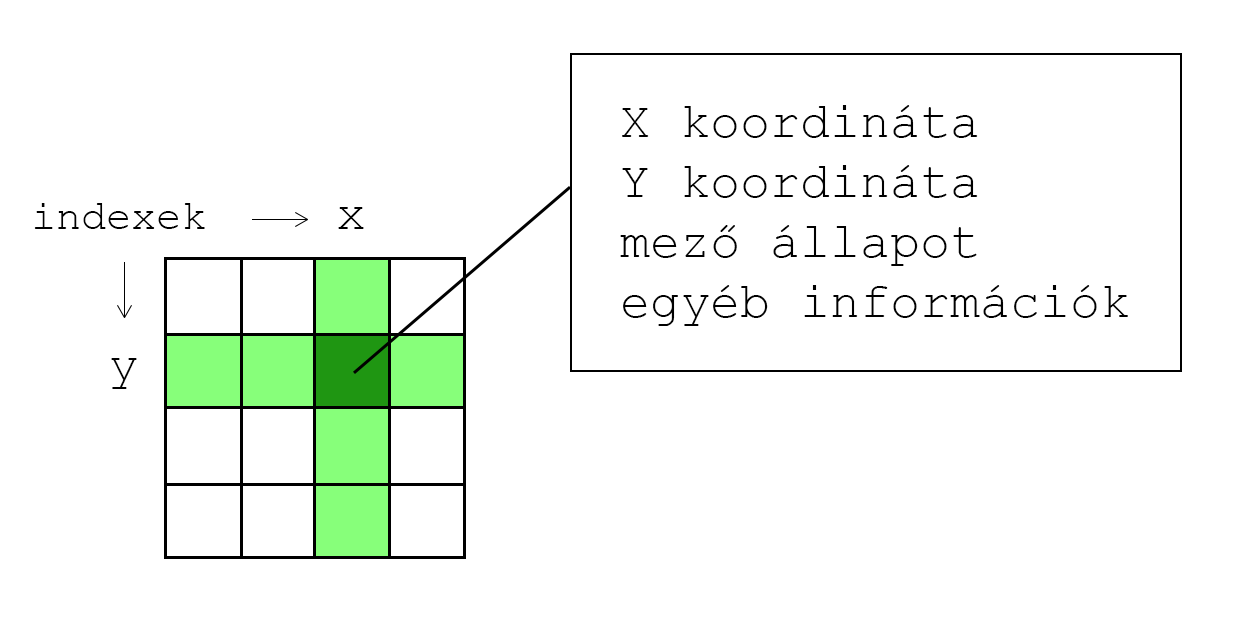
\includegraphics[width=0.6\linewidth]{kepek/field-representation.png}
	\caption{\textit{Tábla reprezentáció}}
	\label{fig:field-repr}
\end{figure}

A mezők állapotai az alábbiak lehetnek:
\begin{itemize}	
	\item 0 - semleges
	\item 1 - kezdő játékos
	\item 2 - másik játékos
	\item 3 - tiltott mező
	\item 4 - csapda mező
\end{itemize}

Fontos különbséget tennünk az index és a koordináták között. Az index az elméleti, a koordináták a fizikai elhelyezést jelölik. Utóbbi a kirajzoláshoz szükséges.

Tehát a 2. sor 3. oszlopában található mező állapotára így hivatkozhatunk: \\
\texttt{mező[3][2].állapot}.

\SubSection{Szabály ellenőrzés}

Az első dolog, amit meg kell vizsgálnunk, amikor egy játékos letesz egy karaktert, a mező állapota. Ilyenkor lekérjük a kiválasztott mező indexeit, majd ez alapján kikeressük a mező értékeinket tároló objektumból a mező állapotát. Ha a mező semleges, kirakjuk a mezőre a karaktert. Ha csapda, akkor annak megfelelően járunk el. Ha már egy játékos karakterét tartalmazza, vagy a mező tiltott, nem történik semmi, nem kerül ki a karakter, a játékosnak másik mezőt kell választani.

Ha sikerült kitenni a karaktert, ellenőriznünk kell, hogy nem nyert-e a játékos. Ránézésre ugyan nyilván való, és egy szempillantás alatt látszik az eredmény, de hogy magyarázzuk el a számítógépnek?

A nyertes kombinációk kijöhetnek vízszintesen, függőlegesen, vagy átlósan (ebből kettő is van). Tehát ezeket a vonalakat kell megnézni. Ezt tehetjük úgy is, hogy végig nézzük az összes ilyen vonalat, hogy van -e nyertes kombináció a táblán. Egy nagy pálya esetén ez illetlenül erőforrás igényes lenne. Mivel minden karakter lerakást ellenőrzünk, így elég mindig csak a legutoljára letett karaktert és környezetét vizsgálni. Így a vizsgálandó területet máris lecsökkentettük egy $9 \times 9$ nagyságú négyzetre. Elkezdjük számolni a játékos karakterét, ha elérjük az öt egyforma karaktert, a játékos nyert. Ebben az esetben az ellenőrzést megszakíthatjuk, nincs már szükség a többi irány ellenőrzésére. Előfordulhat azonban, hogy az öt egyforma karakter nem egymás mellett helyezkedik el, ezért, ha olyan karakter következik, ami különbözik, a számlálót 0-ra kell állítani.

Még egy szempont az ellenőrzés során a pálya széle. Ebben az esetben a vizsgálandó terület túlnyúlhat a pályán, és ebben az esetben az indexek negatívvá válhatnak, így nem létező indexű elemeket keresnénk. Ennek kiküszöbölésének egy módja, ha minden irány ellenőrzése előtt kiszámoljuk az érintett mezők kezdő és záró indexekeit a pályán, és csak ezeken iterálunk végig. Erre nehéz általános képletet adni, így én mégis megengedem a negatív indexeket, de az ilyen mezőket kihagyom az ellenőrzésből,  ill. nem nyertes mezőként kezelem.


\Section{Klasszikus dáma}
A dáma a világon az egyik legkedveltebb, két személyes, táblás társasjáték, amelyet $8 \times $8-as vagy $10 \times 10$-es méretű négyzetrácsos táblán játszanak lapos, korong alakú bábukkal. A táblát gyakran szokták sakk táblával és a sakk bábuk gyalogjaival helyettesíteni.

\SubSection{Játékszabály}

A játék előtt a bábukat úgy kell elhelyezni, hogy játékosonként 2 vagy 3 sorban a sötét mezőkön helyezkedjenek el, úgy, hogy a sor összes sötét mezőjét kitöltsék. A játékot a fekete kezdi.

A kezdetben felállított bábukkal csak átlósan előre léphetünk, azonos színű mezőre, \ref{fig:checkers_board1} ábra. Ezt a lépés rendszert tovább fejleszthetjük azon bábuk esetében, amelyeket sikerül átvinni a tábla túlsó végébe. Ekkor a bábú dámává válik. A dámák abban fejlettebbek, hogy léphetnek és üthetnek hátrafelé is.

\begin{figure}[!h]
	\centering
	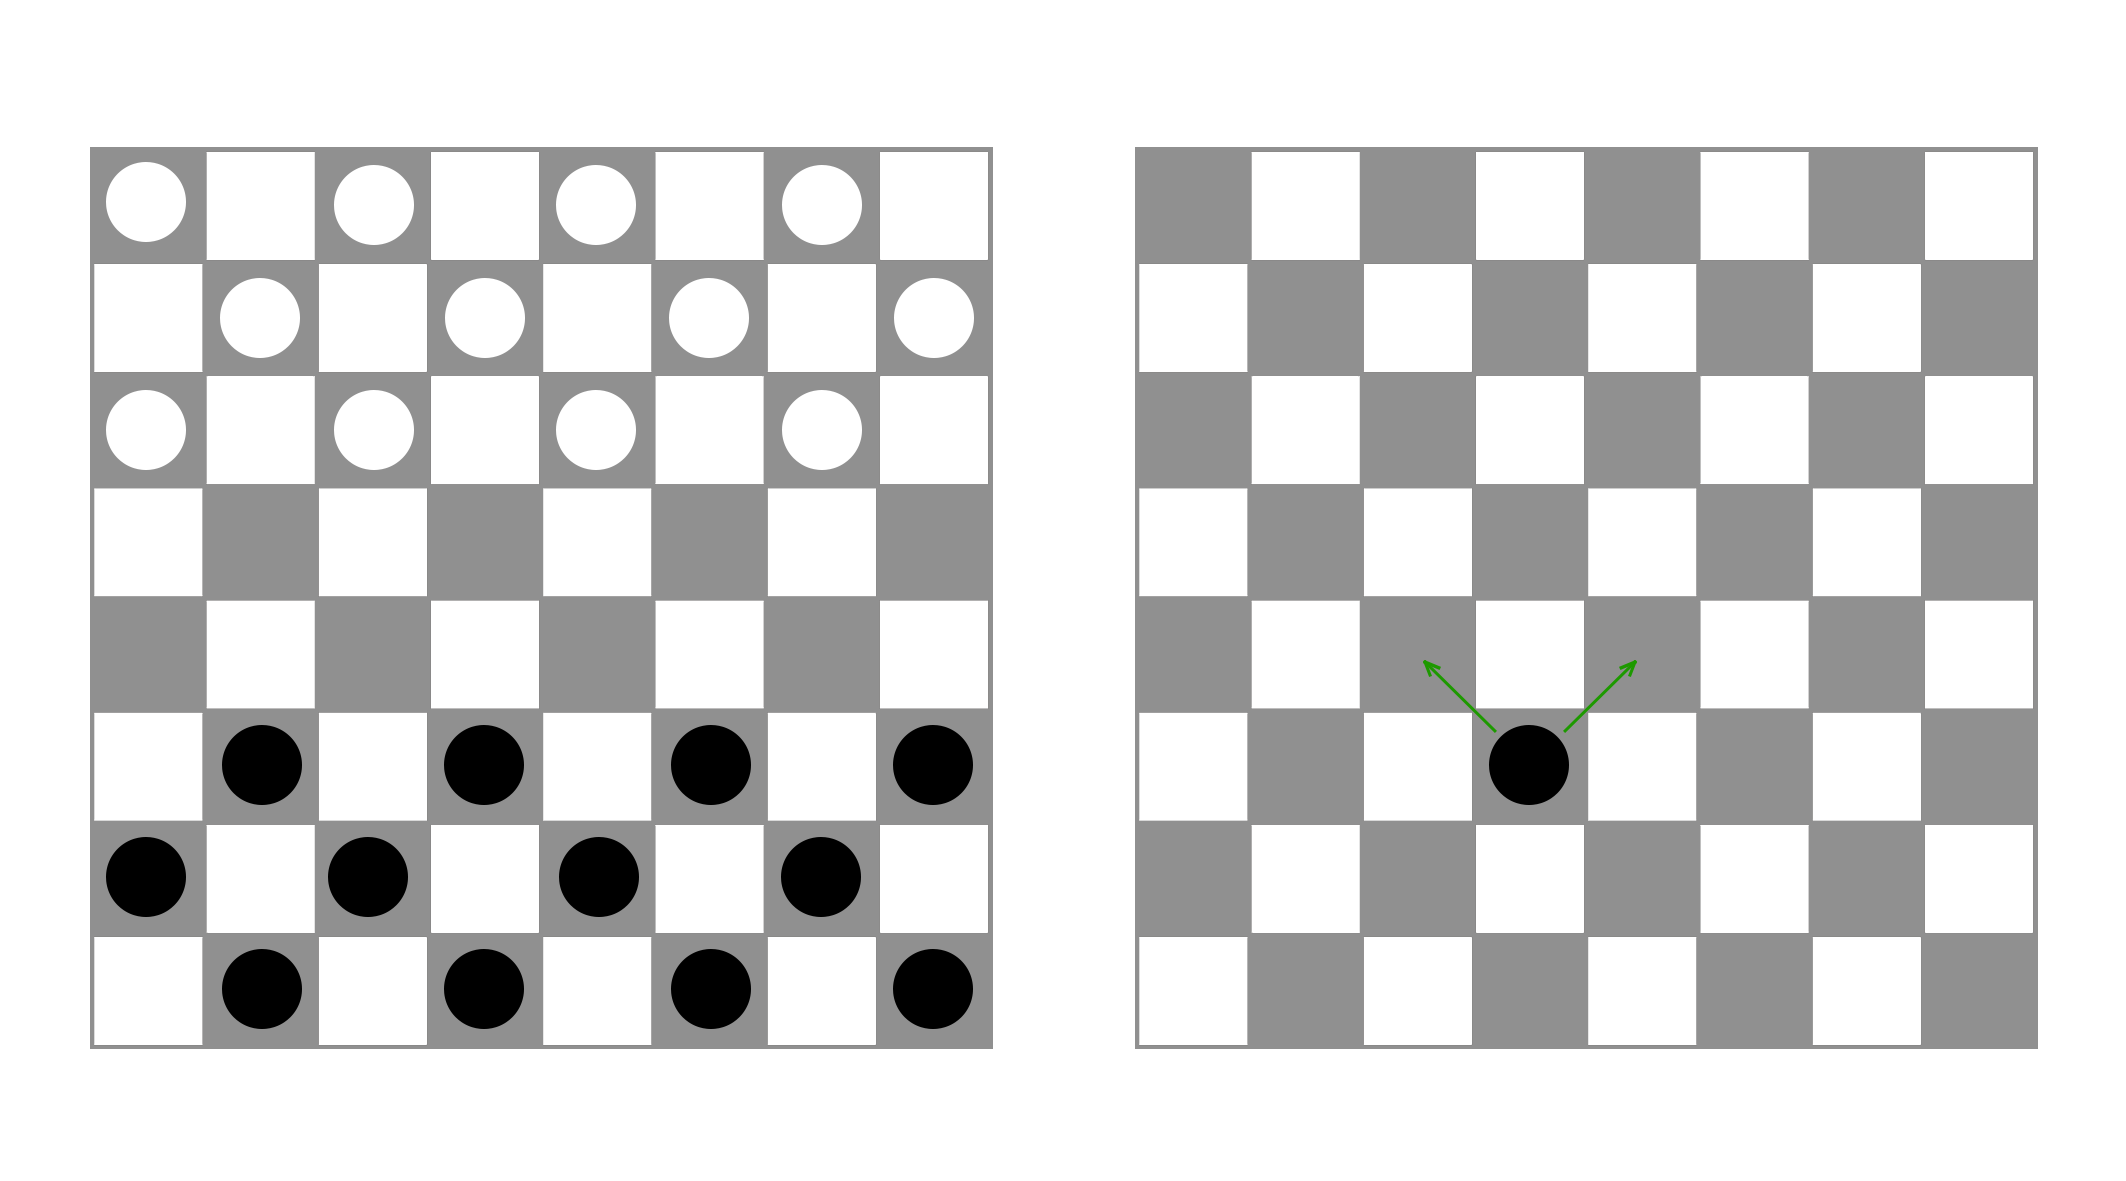
\includegraphics[width=0.8\linewidth]{kepek/checkers_board.png}
	\caption{\textit{Kezdő tábla és lépés egy bábúval}}
	\label{fig:checkers_board1}
\end{figure}

Ha egy bábú útjába kerül egy ellenséges bábú, (tehát előtte átlósan található egy), és a bábú mögött szabadon van egy hely, ütéskényszerbe kerül. Tehát át kell ugornia, és levennie az átugrott bábút. Ha az ugrás után ismét ütéshelyzetbe kerül, a következő bábút is le kell vennie. Ezt pedig addig ismétli, amíg ütési lehetősége van. Ez \textit{ütéssorozatnak} nevezzük, \ref{fig:checkers_board2} ábra. Ha a játékosnak több ütési lehetősége is van, akkor szabadon eldöntheti, melyik ütést hajtja végre.

\begin{figure}[!h]
	\centering
	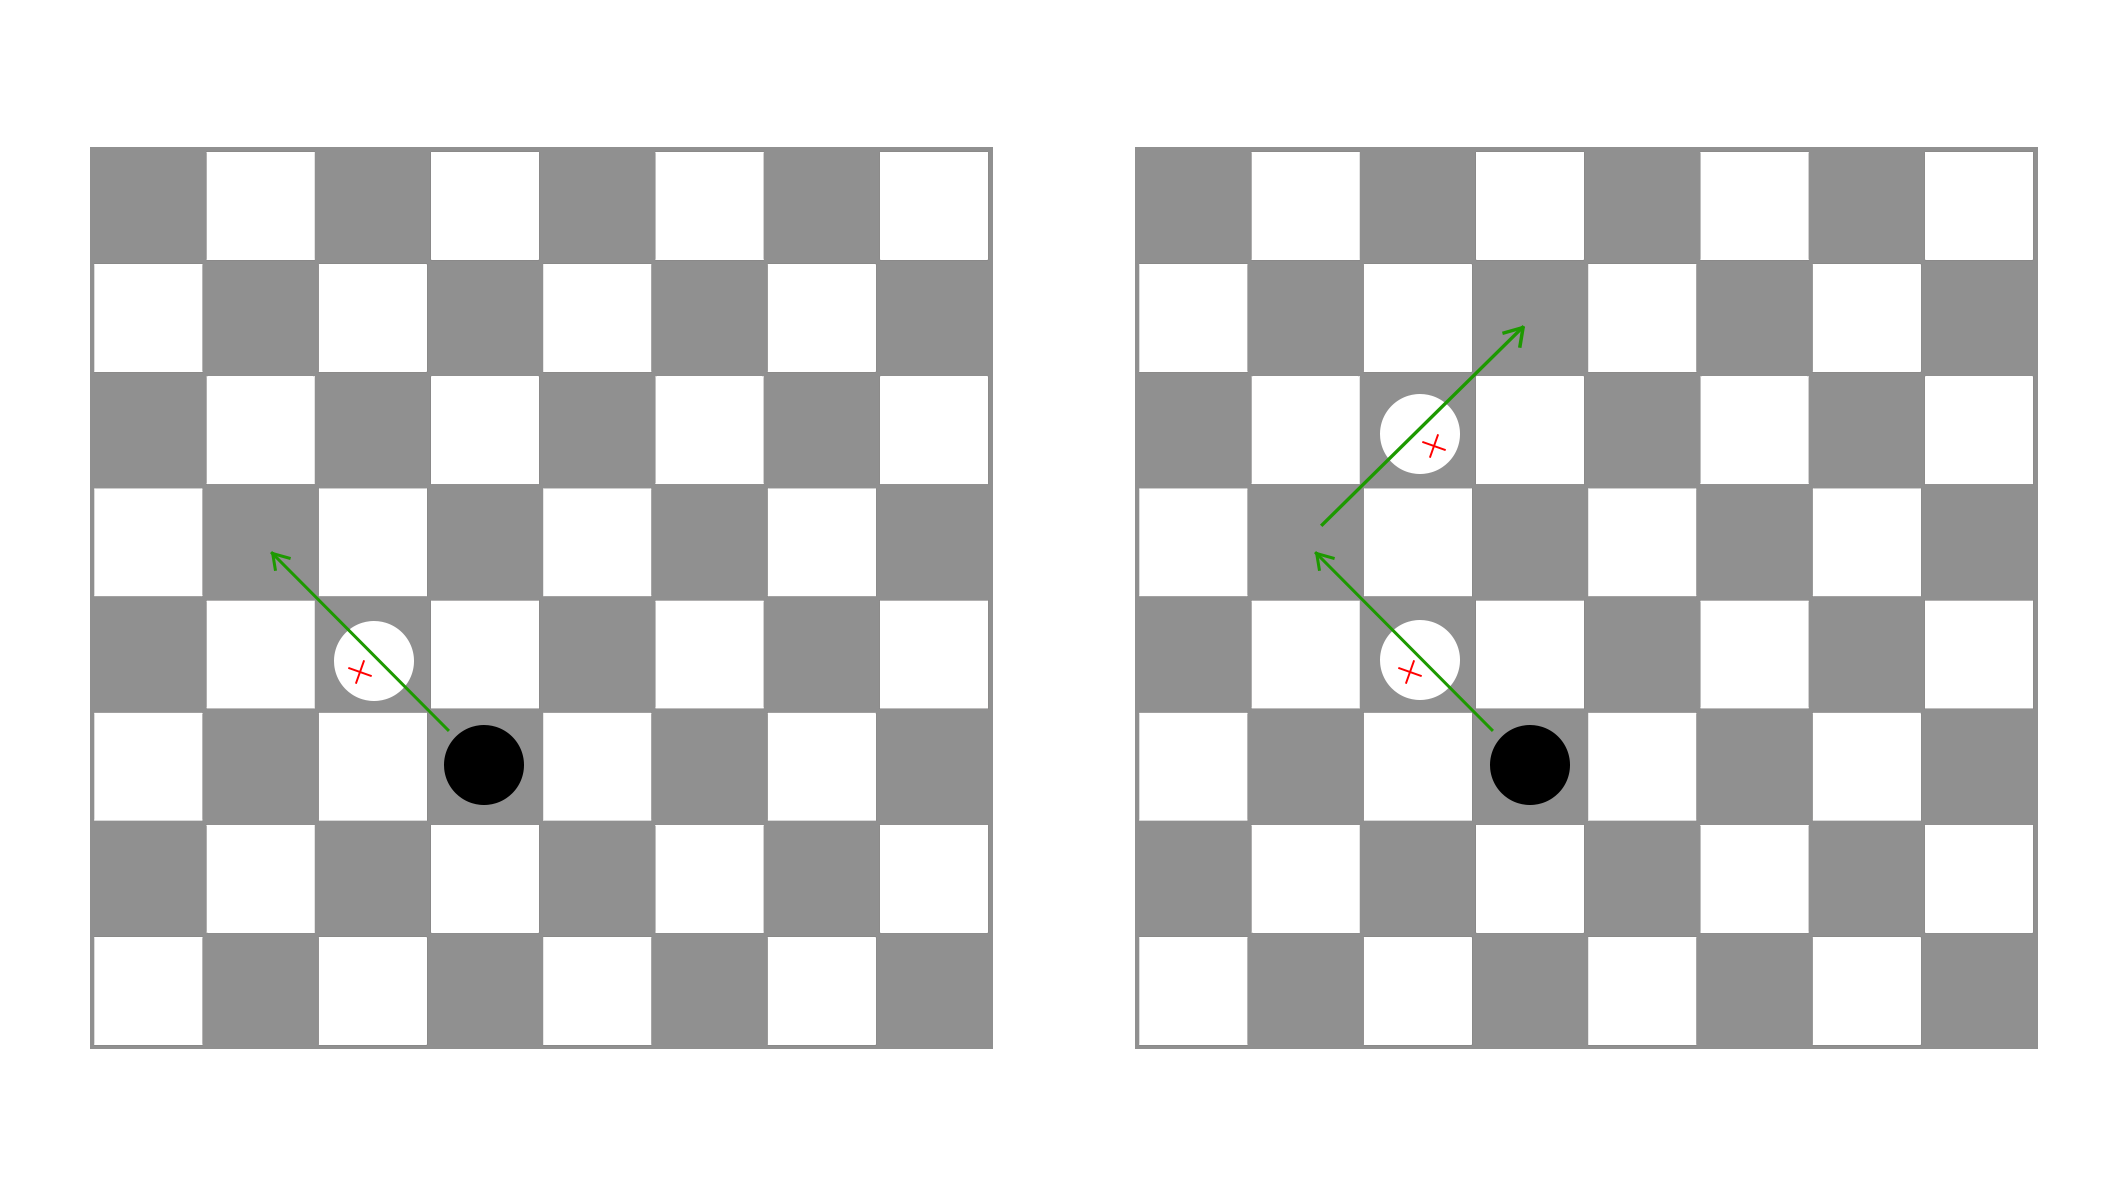
\includegraphics[width=0.8\linewidth]{kepek/checkers_board2.png}
	\caption{\textit{Kezdő tábla és lépés egy bábúval}}
	\label{fig:checkers_board2}
\end{figure}

Előfordulhat, hogy egy bábú az ütéssorozat részeként ér az utolsó sorba, ekkor dámává válik, és ha dámaként újabb ütésre van lehetősége, azt is el kell végeznie.

\SubSection{Variációk}

Alkalmazhatunk a játékban egy olyan szabályt, amely szerint a játékos \textit{"nekifutásból" üthet}. Erre 3 változat létezik:

\begin{itemize}
	\item Az ütés előtt, a leütött bábu előtt tetszőleges számú üres mezőt átugorhat.
	\item Az ütés után, a leütött bábu mögött tetszőleges számú üres mezőt átugorhat.
	\item Az előző két módszer kombinációja.
\end{itemize}

\SubSection{Nyertes}

A játékot az nyeri meg, aki az ellenfelét lépésképtelen helyzetbe hozza, vagy az ellenfél össze bábúját leütötte \cite{checkers-rules}.

%forrás: http://mek.oszk.hu/00000/00056/html/133.htm

\SubSection{Személyre szabhatóság}

A dámában az egyéni változtatások mellett néhány, az amőbában említettet is érdemes alkalmazni.
\begin{itemize}
	\item Csak dámák:
	
	Már a játék kezdetekor minden bábu dáma. Tehát hátra felé is léphet és üthet.
	\item Nekifutás:
	
	A játékszabályzatban szó volt a "nekifutásból" ütés 3 formájáról. Hogy lehessen -e nekifutás, és ha igen, akkor melyik, ennek eldöntését a játékosok eldönthetik akár maguk is.
	
	\item Csapda mezők:
	
	A pályán olyan mezőket helyezünk el véletlen szerűen, amelyekre, ha karaktert tesznek, a karakter kitörlődik (végez vele a csapda).
	
	\item Elhelyezhető csapdák
	
	A játék kezdetekor mindkét játékos kap néhány karaktert, amelyet letéve csapdát helyezhet el.	
\end{itemize}

Ahogy az amőbánál, úgy a dáma játék esetében is megjelennek így nem determinisztikus vonások a szabályrendszerben. A tábla mérete véges marad, viszont a lépés irányára vonatkozó szabályok lazításával a játszmák hossza is változik. A csapdák elhelyezésének a lehetőségével a teljes információs jellege változik a játéknak.

